\documentclass[conference]{IEEEtran}

\usepackage{cite}
\usepackage{amsmath,amssymb,amsfonts}
\usepackage{algorithmic}
\usepackage{graphicx}
\usepackage{textcomp}
\usepackage{xcolor}
\graphicspath{ {./pics/} }

\def\BibTeX{{\rm B\kern-.05em{\sc i\kern-.025em b}\kern-.08em
    T\kern-.1667em\lower.7ex\hbox{E}\kern-.125emX}}
\begin{document}

\title{meet\&do: Meeting website for students and enthusiasts\\}

\author{\IEEEauthorblockN{Stanislas Lange}
\IEEEauthorblockA{\textit{Dept. of Computer Science} \\
\textit{Hanyang University}\\
Seoul, South Korea\\
stanislas@hanyang.ac.kr}
\and
\IEEEauthorblockN{Simon Gaussmann}
\IEEEauthorblockA{\textit{Dept. of Industrial Engineering} \\
\textit{Hanyang University}\\
Seoul, South Korea\\
simongaussmann6658@web.de}
\and
\IEEEauthorblockN{Stéphane Rabenarisoa}
\IEEEauthorblockA{\textit{Dept. of Computer Science} \\
\textit{Hanyang University}\\
Seoul, South Korea\\
rabena.stephane@gmail.com}
\and
\IEEEauthorblockN{Marc-Antoine Dariel}
\IEEEauthorblockA{\textit{Dept. of Information Systems} \\
\textit{Hanyang University}\\
Seoul, South Korea\\
marc-antoine.dariel@cpe.fr}
}

\maketitle

\begin{abstract}
meet\&do is a website that aims to put people in touch who have similar interests and hobbies or need help with issues related to their studies. Enthusiasts can find each other through the website and share real-life activities together.
\end{abstract}

\section{Introduction}

Nowadays, we are more connected than ever through social media and all kinds of internet-based services yet somehow people are still isolated from each other. Forming friendships and relationships has become challenging for some as it is easy and convenient to hide behind a social media profile. Everyone has an online presence. In this environment, many may find themselves looking for real-life interactions.

We want to create a website that aims at putting people in touch who have similar interests and hobbies or need help with issues related to their studies. Getting in touch online is easy but that is just the first step. After finding people with the same interests and making appointments, users of our website meet in real life. Meeting new people works best if you are already interested in similar fields and activities and we want to put people together who have those in common. Common interests to bond over and meet up again in the future or form new friendships.

Where already existing alternatives might take a more generic approach, we want to create a solution that gives users the opportunity to choose what they are looking for from the beginning. Therefore, the website will be divided into four main areas. That makes it less confusing and easy and intuitive to navigate.

\section{Alternatives}


\subsection{Jodel}

Jodel is a Social Media platform from Germany that aims particularly at university students and connecting people who are in the same area. User’s can share content, however events as such can’t be created. It is only available on mobile operating systems and has no website. Users in an area can’t see posts other than those made locally. Posts are assigned colors which are chosen randomly. The platform is available in several languages and European countries.

\subsection{Meetup.com}
 Meetup is the competitor with the most similarities to our project. The website offers a service used to organize online groups that host real life events for people with similar interests. Events of all kinds can be hosted which don’t have to conform to certain categories. Also, event organizers have to pay a fee to host events. The website is available in many languages.

\subsection{Others}
Various other social networks like Facebook that also include the feature to create and host events. In essence, all social media platforms fulfill similar functions that aim at communication and gathering people. Some of them, like Facebook, have inbuilt Event Managers to create and host events. Others, like Instagram and Twitter, allow users to track events and participating people via hashtags.

Differentiating aspects of MeetnDo: While Jodel restricts the user’s view to their local area and is not suitable to host events, our project aims at events that can be hosted anywhere the user chooses and offering a clear and user friendly interface which is color coded by event type for a more organized experience. Also, Meetup.com takes a wider and more generic approach which is something we want to avoid in order to make the service more accessible and less overwhelming. For that reason our service offers preset categories that make it easy for the user to determine whether they are potentially interested in an event.

\section{Technical specification}

\subsection{Software used}

The website will be built using Ruby 2.6 and the framework Ruby on Rails 6.0. We chose Ruby and Rails because we like the simplicity of the language and we want to expand our knowledge on this framework. Ruby on Rails allows us to save time for CRUD (Create, read, update and delete) operations and allows us to focus on feature that differentiate our website. Moreover, Ruby on Rails follows the MVC architecture (Model, View, Controller) which will help us keep our code clean and organized in a specific folder arborescence and separate our code depending on its use (models, controllers, routes, helpers, and so on.

Rails also enables us to implement a REST API which can be used if we use a front end Javascript framework like Vue.js or if we end up working on a mobile app. The REST API would use JSON and would be a layer above the CRUD operations.

For the version controlling system, we chose git hosted on the GitHub service. Our repository is public so we don't have any limitation and we are able to be four collaborators on it. We use GitHub's board feature called "Projects" to organize our project with a Kanban-like workflow management method. We have a board for this very paper called "Documentation" and an other one for the actual implementation which will help us keep track of what's been done when coding the website.

For the development environment half of our team is using macOS and the other half is using Windows 10. Our text editor of choice is VS Code.

\subsection{Hosting}

Our stack only requires Ruby and a DBMS (Database Management System) which is PostgreSQL. For this matter, we chose Heroku which is a hosting provider focusing on easing the deployment process for the developers. Thus, we will be able to deploy our code to a development environment or production environment via the command line using Heroku as a Git remote or via the Heroku CLI (Command Line Interface) client.

The deployment can also be made from GitHub using their new CI/CD system called GitHub actions, from which we can deploy to Heroku using the Heroku Action which is a wrapper for the CLI. This helps keeping track of the deployments made and ensures the code running is the one in the version control system.

For our initial release we don't expect a very high number of users, hence the choice of the free plan for Heroku as well as Heroku's managed service. The only cost for now would be the domain name which costs about \$10/year.


\section{Role assignment}

\begin{tabular}{ |p{0.2\linewidth}|p{0.15\linewidth}|p{0.45\linewidth}| }
\hline
Role & Name & Task description and etc. \\
\hline
User & Marc-Antoine & Quality assurance, testing of the product as a normal user through multiple device \\
\hline
Customer & Simon & Ensuring requirements are the most precise possible, and that they stay up to date during the lifetime of the project \\
\hline
Software developer & Stanislas & Implementation of the requirements and technical feedback \\
\hline
Development manager & Stephane & Work distribution and time, deadline management. Communication management with the client. \\
\hline
\end{tabular}

\section{Requirements}

\subsection{Sign-up page}

The sign-up section should show these fields:

\begin{itemize}
    \item First Name
    \item Name
    \item Gender
    \item Date of Birth
    \item Email
    \item Password
    \item Password confirmation
    \item Anti-robot Captcha verification
    \item Sign up button
\end{itemize}

When the user presses the sign-up button considering all
the information given is valid, the user must click the verification link sent by email to create his account and have access to the home page.

\subsection{Login page}

The login section should show 2 fields: username and password fields as well as a login button.

\subsection{Home page}

Once the user created his account or correctly logged in, he should have access to the home page.

The website should be able to localize the user city precisely and state it on the Home page. It also should give the user the possibility to change his location from a list of registered cities in the world.

The user should be able to log in from a Login button at the top right of the home page (if not logged in). The login section should show 2 fields: username and password fields as well as a login button.

The user should be able to log out from a Logout button at the top right of the home page (if logged in).

If the user is not logged in and tries to access to logged in user sections (such as personal information) the access will be denied and Login section will be highlighted to inform the user to sign up or log in in order to access this section.


\subsection{Feed section}

A search bar allows the user to search for a particular meeting.
The home page should show a feed of meetings. The feed should only show non-archived meetings, be sorted from the nearest upcoming date at the top of the page to the latest date at the bottom of the page. The feed should show all types of meetings.

The meeting cards should show:

\begin{enumerate}
\item Name and/or Type: Restaurant
(Lunch/Dinner/Brunch...), Sport (Tennis/Football/Swimming...), Study Lesson (Chemistry/Mathematics/Economics...), Entertainment (Theater/Outdoor show/ Concert...), Art Practice (Painting/Music...)
\item Location: Precise location with exact address and redirection to google maps when address is clicked
\item Time and duration: Meeting time and expected duration
of the activity
\item Price: Can be undefined if free activity or if the price is
not equally shared
\item Current participant number, expected participant
number, max participant number: expected and participant numbers are not mandatory information.
Possibility to click on current participants to display the
list of current participants and access to their profile
\item Details: Text field with additional details from the meeting organizer, the details should be
expandable/collapsible if too long.
\item Visual: Most precise visual describing the meeting, it can
be a promotional photo of a restaurant, the poster of a show, an illustration of Mathematics, ... Whatever visual that can describe the meeting type the most precisely possible
\item Ask to Join Button: This button will open a new window with a message to send to the meeting organizer for joining the meeting. A default message is proposed to the user, but he can make his own. Join and Cancel Buttons available.
\item Remove from feed button: A little cross at the top right of the card that removes the card from the feed
\end{enumerate}

\subsection{Search Filters}

The filter section should give the user the possibility to filter the feed results considering:

\begin{enumerate}
\item The type of meetings
\item The Date/Time of meetings
\item The Duration of meetings
\item Number of participants
\item A location filter (km radius from his current
location)
\item Reset all filters
\item Filter button
\item Restore removed meetings
\end{enumerate}

\subsection{User section}

The user section should give the possibility to the user to
access his personal profile page and settings. Each user has a public profile with a limited set of information such as their name, profile picture, location and past meetings they participated in. An edit page is available for them to update these public details.

Private information such as email, password, account deletion, etc. are available on a different page called account settings.

\subsection{Chat section}

This page should let a user talk to other users via private
messages.

A left column should contain a list of people that the user
has already contacted, and a right column should contain an opened chat between the current user and another user.

The user’s list should display full names and user profile photos. Next to each users' names, something should let the current user know that a user has sent a new message that he/she has not seen already.

The opened chat should contain all messages sent by people included in the chat. The current user should be able to see his/her messages on the right side. Next to each message, a user should be able to see the time (hour format) of receipt of a message.

\subsection{User’s meeting section}

From the user section, which is a menu on the homepage
the user can select a page with all his personal meetings that he is participating in or has shown interest in participating in. This page is called My Meetings. It can be found under this name in the user section.

The basic structure of this page is a list of all the user’s events. All events all displayed chronologically in a timeline format. The user is able to scroll through the timeline and search all content by keywords or different filters.

Other requirements for the My Meetings page:

\begin{enumerate}
\item A search bar on top of the site to search through all of the
user’s meetings (past and upcoming)
\item Meetings can be searched by keywords, location, type of
meeting, tags of a meeting
\item Drop down menu next to the search bar to choose what
type of content is displayed
\item Show all meetups
\item Timeframe (choose between past and future
events)
\item Type of meeting (4 main categories)
\item Only show favorite meetups
\item Show archived meetups
\item On the right side of the bar there is a timeline that indicates dates of meetings, user can scroll through the timeline to navigate the page faster
\item Meetings are listed along the timeline with their individual dates as they occurred
\item All meetings are displayed in chronological order (the most recent first)
\item Different colors for different types of meetings, same as on the homepage
\item The user has the ability to highlight certain meetups which are then given a more prominent location on the page
\item Highlighted meetups are marked as favorites and pinned on top of the page, regardless of their dates
\item User’s favorites can be past events as well as upcoming ones
\item The ‘highlights’ section on top of the page is visibly separated from the rest of the chronologically displayed events
\item Users have the ability to remove meetups from their personalized My Meetings page by “leaving” a meetup
\item In the same way meetups are added to the My Meetings page by ‘joining’ a meetup
\item Users have the ability to archive past events without leaving them, archived events don’t show up on the My Meetings timeline
\end{enumerate}

\subsection{Page for an individual meeting}

From the My Meetings page as well as the Home Feed users can access the page of each individual meeting by clicking on its card in the Feed or My Meetings page.

The page for a certain meeting displays all relevant information added by the creator of the meetings as well as a chatroom and list of people who joined.

\begin{enumerate}
\item All relevant information as well as a title picture are displayed on a blackboard on top of the page (type of meetup, description, location, date, for how many people is planned, etc)
\item Underneath there is a chatroom to which everyone who joined the event has access to
\item All users can access the event page and read information but only users who participate are able to join the chat
\item Users have to ability to ask questions to the creator of a meeting prior to joining
\item On the page of the meeting users have the ability to join the meeting, mark the meeting as “I am interested”, or share a link to the event via social media
\item Users have to ability to hide an event from their home feed if they choose to
\end{enumerate}

\subsection{Create new meeting}

This page should present a form to create a new meeting
which the user will be the organizer of. Required information should be the name of the event (text field), the type of meeting (choose one from a list), the date of the meeting (normalized calendar date) and the meeting location (address from google maps, should be the most accurate possible).

Other information such as the duration of the meeting (numerical value in minutes), the price of the meeting (in local asset, undefined if not stated, otherwise numerical value), the expected and maximum number of participants (numerical values) and some additional details on the meeting (text field).

The form should have a create button as well as a cancel Button. The create button will trigger a confirmation window summing up all the given information and asking the organizer to confirm the meeting creation or go back to editing the meeting. If the organizer confirms the meeting creation, it will create the meeting and it will be uploaded to all the other users meeting feed (in the region). The cancel button should reset the form.

A visual for the new meeting card will be automatically uploaded from a bank of images, the chosen image will have to be the most accurate possible regarding the meeting.
Once the meeting is created, a chat group for this meeting will be created in the chat section. The organizer is basically the administrator of this chat group and each time a new participant will ask to join the meeting, the organizer will
have to either accept/deny his participation from this group chat.
Once the meeting is created, a card will be added to the user’s ‘My meetings’ page and only the organizer will be able to edit or delete the meeting.

\section{Specification}

\subsection{Create new meeting}

On this page, the user has to fill a form with fields corresponding to the following:

\begin{enumerate}

\item Name (required): Text field, maximum 50 characters, only alphanumeric
\item Type (required): 2 Drop-down menus, 1 for the main category, can only select one item between (Sport, Outdoor, Entertainment, Culture, Food, Education), this selection is required

The 2nd drop-down menu will be updated depending on the choice of the 1st drop-down menu, can only select one item, this selection is not required (‘----’ if nothing is chosen)

A ‘Other’ item is present in the 2nd drop-down menu list, if selected a new text field will appear (20 characters, only alphanumeric) with precision of the item written by the user, not required.
\item Date (required): A text field which is not editable by the user, next to it a button with a calendar icon, when the user clicks on the field or the calendar icon, a new calendar pops out with previous dates in gray (not selectable), user can navigate through the years, months and select the date, when selected, the calendars hides and the text field is filled with the selected date.
\item Time (required): Drop down menu, items are all daily hours in a 15 minutes separation, user has to select one item.
\item Location (required): Search bar coming from google locations API, user will type the location name and a list of locations known by google will appear (autocomplete), user has to select one, a button next to the text field with a map icon is also available, when clicked, a map will pop up and the user can drag a pointer to the location, if the given point doesn’t correspond to any of the google API’s location, the location will be updated as cardinal coordinates.
\item Duration: Text field with only numeric characters accepted, from 0 to 1440 (24 hours), if text field is not filled in, it is considered as ‘undefined’.
\item Price: Price per participant, text field with only numeric characters accepted, from 0 to 999999999999999, if text field is not filled in, it is considered as ‘undefined’. The asset used is the one from the country of the set location.
\item Expected participants:Text field with only numeric characters accepted, from 0 to 999999999, if text field is not filled in, it is considered as ‘undefined’.
\item Maximum participants: Text field with only numeric characters accepted, from 0 to 999999999, if text field is not filled in, it is considered as ‘undefined’.
\item Details: Text field, details are to be written from the organizer, 5 lines of text max, only alphanumeric characters.
\item Create Button: Opens a new page with all the form but the information are not editable (grayed areas), the only editable field is the picture of the event (selected in the google bank of images depending on the type and location of the meeting). The user can select the graphic used from this bank of images that will appear in the meeting card. The user can then Confirm? Yes/No, if No, back to the form, the new page pops out, if yes meeting is created and back to home page.
\item Cancel Button: Resets the form after alerting the user with an alert box (Confirm? Yes/No) if confirmed
\end{enumerate}

\subsection{User’s meetings section}

\begin{enumerate}
    \item Header with MeetnDo logo and MyMeetings title
    \item White page background
    \item Search bar
    \begin{enumerate}
        \item Search bar on top of the page to search meetings by keywords
        \item Results are drawn from a database of all of the user’s past and present meetings
        \item When executing a search results are displayed as a list on the MyMeetings page
        \item Users can click on the result to reach the page of the individual meeting
        \item Feature to to guess the user’s search request by keywords, associated meetings are recommended (auto-complete for search requests)
    \end{enumerate}
    \item Meetings can be searched by keywords, location, type of meeting, tags of a meeting
    \item Ability to filter search result
    \begin{enumerate}
        \item Drop down arrow next to the search bar to filter what results are displayed
        \item Implementation of checkbox selection filter (by clicking downward arrow user is taken to the checkbox selection)
        \begin{enumerate}
            \item Show all meetings checkbox selected by default
            \item Checkbox to select type of meeting (Food, Study, Sports, Activities)
            \item Checkbox to filter by location (select nearby, my area, all)
            \item Checkbox to select the timeframe (only show past meetings, only show future meetings)
            \item Checkbox to only show meetings marked as favorites
            \item Checkbox to only show archived meetings
        \end{enumerate}
    \end{enumerate}
    \item Timeline on the right side of the MyMeetings page
    \begin{enumerate}
        \item User can move through the timeline by scrolling on the page
        \begin{enumerate}
            \item Marker on the timeline indicates the current position/date
            \item User’s have the ability to navigate the page faster by clicking and dragging the marker across the timeline or scrolling directly on the timeline
        \end{enumerate}
        \item Buttons to show more/ show less (+ or -) on top of the timeline to select the scope of the timeline
        \begin{enumerate}
            \item Enables the user to switch between Years/Months/Days to control the level of detail on the timeline
            \item Purpose: more organized MyMeetings page in case multiple meetings for a specific date, more organized overall display for many meetings
        \end{enumerate}
        \item Meetings are listed along the timeline as they occurred
        \begin{enumerate}
            \item Listed chronologically by default
        \end{enumerate}
    \end{enumerate}
    \item  Meetings on the MyMeetings page are displayed in boxes
    \begin{enumerate}
        \item Box includes title of specific meeting in bold letters
        \item Short, general descriptions as preview that users choose when creating a meeting
        \item Location of meeting
        \item Indicator for rough amount of people attending/ interested in specific meeting e.g. <10, 10+
        \item Boxes feature slightly rounded corners
    \end{enumerate}
    \item Different colored boxes for a well arranged layout and usability
    \begin{enumerate}
        \item Distinguished by the 4 general types of meetings
        \begin{enumerate}
            \item Red for Food
            \item Yellow for Education
            \item Light Green for Sports
            \item Dark Green for Outdoor
            \item Orange for Culture
            \item Blue for Entertainment
        \end{enumerate}
        \item Hex transparency 50\%
    \end{enumerate}
    \item ‘Highlights’ section pinned above the regular timeline view
    \begin{enumerate}
        \item User has the ability to mark meetings as favorites
        \begin{enumerate}
            \item Star symbol in the right corner of every meeting box
            \item By default only outlines, by clicking the star is displayed yellow thus marked as favorite
        \end{enumerate}
        \item ‘Highlights’ section visibly divided from the rest of the timeline by light yellow background
    \end{enumerate}
    \item Controls over content shown on MyMeetings page
    \begin{enumerate}
        \item Ability to remove meetings from MyMeetings
        \begin{enumerate}
            \item Leave specific meeting via right click or designated button on the page of the individual meeting
        \end{enumerate}
            \item Ability to add meeting to MyMeetings
        \begin{enumerate}
            \item Via right click on homepage or designated button ‘Join Meeting’ on the page of the individual meeting
            \item Mark meeting as ‘I’m interested’ on the individual page of the meeting
        \end{enumerate}
        \item Ability to archive past meetings without leaving
        \begin{enumerate}
        \item By right click or designated button ‘Archive’ on the page of the individual meeting
        \item Archived meetings are not shown on the timeline of MyMeetings but can still be searched for
        \item Archived meetings are displayed with grey background
        \end{enumerate}
    \end{enumerate}
\end{enumerate}

\subsection{Page of an individual meeting}

The page of each individual meeting contains all relevant information about the event. Users can access the page from anywhere e.g. from the Home Feed, MyMeetings or a user’s profile by simply clicking on the box or the title of a specific meeting. All users are able to access the page of a meeting.

\begin{enumerate}
    \item Background of the page is shown in the same color as the meeting box but at 10\% opacity
    \item Title of the meeting on top of the page in bold letters
    \item Contains all information about the meeting
    \begin{enumerate}
        \item Type of meeting (as bullet point beneath headline)
        \item Description of the meeting as put in by the creator of the meeting as ‘Details’
        \begin{enumerate}
            \item Text field, Maximum 5 lines of text, alphanumeric characters only
        \end{enumerate}
        \item General information displayed as
        \begin{enumerate}
            \item ‘ When: "dddd, dd MMMM yyyy HH:mm" ‘ as chosen by the creator
            \item Approximate duration is stated underneath date and time, if the creator has provided a duration
            \item Location of the event displayed on the right of time, date and duration
            \begin{enumerate}
                \item Section of the map where the meeting will take place is embedded in the page through Google Maps API/HTML (small window)
                \item Google Maps pin on the map marks the exact location
                \item Written address/location is displayed beneath the Google Maps window
                \item By clicking on the map the user is taken to Google Maps with the event location marked
            \end{enumerate}
            \item Price per participant is displayed underneath as ‘Price: Value’
            \begin{enumerate}
                \item If no price provided, ‘Price’ is not shown
                \item If price is indicated as 0, it is displayed as ‘Price: Free’
                \item If no specific price provided, price can also be displayed as an estimate as chosen by the creator (\$/\$\$/\$\$\$)
            \end{enumerate}
            \item Expected participants as ‘Expected participants: Value’ if provided by creator
            \item Maximum participants as ‘Maximum participants: Value’ if provided by creator
            \item Beneath, the creator/host of the meeting is indicated by displaying a small, circular profile picture as well as the name
            \begin{enumerate}
                \item Users can click on the creator to be taken to the person’s profile page
            \end{enumerate}
        \end{enumerate}
    \end{enumerate}
    \item Underneath the information about the meetings there are buttons the user can click, those buttons are aligned
    \begin{enumerate}
        \item ‘Join’ button to join the meeting
        \item ‘I’m interested’ button to mark as interested in
        \item ‘Join Chat room’ button, only becomes visible once the user has joined the meeting
        \item Links to a chat page of the individual meeting
        \item ‘Share’ buttons from various social media plugins to share on social media platforms
        \item ‘Not interested’ button, on the lower right corner and smaller than the other buttons
        \begin{enumerate}
            \item Meetings marked as ‘Not interested’ will not be suggested to the user again on the Home Feed
        \end{enumerate}
    \end{enumerate}
    \item To exit the page of an individual meeting, click on the small Exit button in the upper right corner (X)
\end{enumerate}

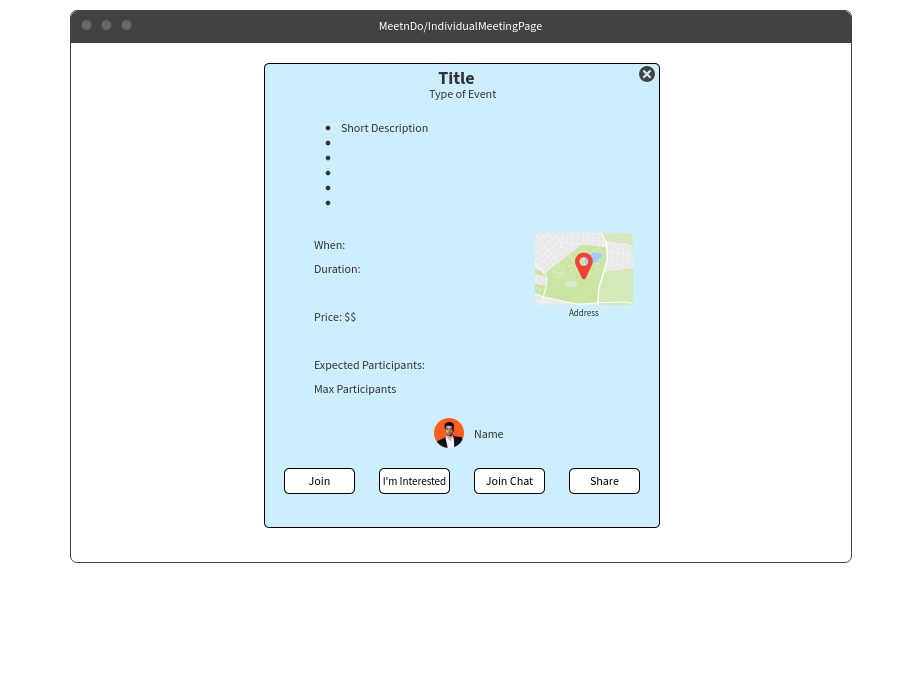
\includegraphics[scale=0.3]{mockups/meeting}

\subsection{Sign-up page}

\begin{enumerate}
    \item With a Google Account
    \item With an email
    \begin{enumerate}
        \item Name --- Text field, 50 characters max, can’t be empty
        \item Email address --- Text field, 255 characters max, unique and can’t be empty
        \item Password --- Text field (password type), 255 characters max, can’t be empty
        \item Confirmation password --- should match the password
        \item Location --- Text field which is auto-completed via an API (or a table in database)
    \end{enumerate}
\end{enumerate}

\end{document}
